


%ICFO poster template
%====================
%
%This is a LaTeX poster template designed to match the existing (powerpoint) poster template for ICFO - The Institute of Photonic Sciences, Barcelona.
%
%This template uses the baposter.cls LaTeX class, available from http://www.brian-amberg.de/uni/poster/
%
%Created by Emilio Pisanty, 2017-2018, based on existing ICFO materials


\documentclass[a0paper,portrait]{baposter}

\usepackage{relsize}         % For \smaller
\usepackage{url}             % For \url
\usepackage{epstopdf}	     % Included EPS files automatically converted to PDF to include with pdflatex
\usepackage{xcolor}
\usepackage[export]{adjustbox}
\usepackage{setspace}
\usepackage{multicol}
\usepackage{amsmath,amssymb}
\usepackage{mathrsfs}        % For \mathscr
\usepackage{array}
\usepackage{multicol}
\usepackage{colortbl}


%%% Global Settings %%%%%%%%%%%%%%%%%%%%%%%%%%%%%%%%%%%%%%%%%%%%%%%%%%%%%%%%%%%

\graphicspath{{Images/}}	% Root directory of the pictures 
\tracingstats=2			% Enabled LaTeX logging with conditionals

%%% Color Definitions %%%%%%%%%%%%%%%%%%%%%%%%%%%%%%%%%%%%%%%%%%%%%%%%%%%%%%%%%

\definecolor{bordercol}{RGB}{40,40,40}
\definecolor{headerfontcol}{RGB}{0,0,0}
\definecolor{icfoblue}{RGB}{41,62,165}
%
\definecolor{icfogreen}{RGB}{161,207,15}
\definecolor{icfogray1}{RGB}{233,233,233}
\definecolor{icfogray2}{RGB}{192,192,192}
\definecolor{icfogray3}{RGB}{116,116,116}
\definecolor{authorgray}{RGB}{89,89,89}

%%%%%%%%%%%%%%%%%%%%%%%%%%%%%%%%%%%%%


%%% Top margin to zero to make the title box reach the top of the paper
\geometry{tmargin=0mm,bmargin=3.5mm,lmargin=9mm,rmargin=9mm}

%%% Sans-serif maths
\usepackage{sansmathfonts}

%%% other options that work OK:
%\usepackage[helvet]{sfmath}
%\usepackage[tx]{sfmath}
%\usepackage[px]{sfmath}
%\usepackage[cm]{sfmath}


%%% Core font - Helvetica instead of Arial because non-xetex TeX doesn't have Arial.
\usepackage[scaled]{helvet}
\renewcommand\familydefault{\sfdefault} 
\usepackage[T1]{fontenc}


\newcommand{\titlefont}{\bf \Huge \color{white}}
\newcommand{\authorfont}{\bf \Large \color{white}}
\newcommand{\headerfont}{\bf \large \color{white}}
\newcommand{\subheaderfont}{\bf \large }
\newcommand{\acknowledgementsfont}{\small}
\newcommand{\footerfont}{\footnotesize}





%%%%%%%%%%%%%%%%%%%%%%%%%%%%%%%%%%%%%%%%%%%%%%%%%%%%%%%%%%%%%%%%%%%%%%%%%%%%%%%
%%% Document Start %%%%%%%%%%%%%%%%%%%%%%%%%%%%%%%%%%%%%%%%%%%%%%%%%%%%%%%%%%%%
%%%%%%%%%%%%%%%%%%%%%%%%%%%%%%%%%%%%%%%%%%%%%%%%%%%%%%%%%%%%%%%%%%%%%%%%%%%%%%%

\begin{document}

\typeout{Poster rendering started}

%%% Setting Background Image %%%%%%%%%%%%%%%%%%%%%%%%%%%%%%%%%%%%%%%%%%%%%%%%%%
\background{} %%% No background

%%% General Poster Settings %%%%%%%%%%%%%%%%%%%%%%%%%%%%%%%%%%%%%%%%%%%%%%%%%%%
\begin{poster}{
    grid=false,
    borderColor=bordercol,
    headerColorOne=icfoblue,
    headerColorTwo=icfoblue,
    headerFontColor=headerfontcol,
    boxColorOne=white,
    headerheight=0mm,
    boxheaderheight=2em,
    headershape=rectangle,
    headerfont=\headerfont,
    textborder=none,
    headerborder=none,
    background=plain,
    bgColorOne=white,
    boxshade=plain,
    columns=2
}
{}{}{}{}  %%%% The standard baposter title settings are not flexible enough, so this sets them empty, and then re-creates them anew inside a standard headerbox.



%%%%%%%%%%%%%%%%%%%%%%%%%%%%%%%%%%%%%%%%%%%%%%%%%%%%%%%%%%%%%%%%%%%%%%%%%%%%%%%
%%%%   Formalities %%%%%%%%%%%%%%%%%%%%%%%%%%%%%%%%%%%%%%%%%%%%%%%%%%%%%%%%%%%%
%%%%%%%%%%%%%%%%%%%%%%%%%%%%%%%%%%%%%%%%%%%%%%%%%%%%%%%%%%%%%%%%%%%%%%%%%%%%%%%

%%%%%%%  Title box.
\headerbox{}{
name=toplogobox, span=2, column=0, row=0, boxheaderheight=0mm, 
	headerColorOne=white,
	headerColorTwo=white,
    boxColorOne=white, 
    boxColorTwo=white,
    boxshade=shadelr
}{
\vspace{5mm}

\includegraphics[width=0.16\textwidth]{Logos/ICFO-trimmed.png}
}

\headerbox{}{
name=titlebox, span=2, column=0, row=0, boxheaderheight=0mm, below=toplogobox,
	headerColorOne=icfoblue,
	headerColorTwo=icfoblue,
    boxColorOne=icfoblue, 
    boxColorTwo=icfoblue,
    boxshade=shadelr
}{
\vspace{4mm}
\begin{minipage}{0.99\textwidth}
\begin{tabular}{p{0.0001\textwidth}p{0.95\textwidth}}
&
\vspace{0pt}
\begin{minipage}{0.94\textwidth}
\raggedright
\setstretch{2.7}
%
\color{white}
\rule{\textwidth}{3pt}

%
{ \titlefont 
%
Title of the project will go here, font Arial Black BT in size Huge 
%
}\\[3mm]
\setstretch{1.5}
\textcolor{white}{
\authorfont
%
Names of authors will go here using the font Arial Bold in size Large
%
}\\[2mm]
\setstretch{1.25}
\textcolor{white}{
\small
%
Affiliation, departments/groups\\
Affiliation, departments/groups
%
}
\end{minipage}
\end{tabular}
\vspace{5mm}
\end{minipage}
}

%%%%%%%%%%%%%%%%%%%%%%%%%%%%%%%%%%%%%%%%%%%%%%%%%%%%%%%%%%%%%%%%%%%%%%%%%%%%%%%

%%% Bottom logos. Typeset at the start because (i) they're a formality, and (ii) the bottom content boxes require this to be defined for the above=bottomlogos option to work.

%%%%%%%%%
%
%  This box contains the trustee logos. This is mandatory for posters which will be displayed in the ICFO foyer, but you can edit or remove it if you're preparing a poster that will be presented externally.

\headerbox{}
{name=bottomlogos, span=2, column=0, boxheaderheight=1.5mm, boxColorOne=white, headerColorOne=white, headerColorTwo=white, above=bottom}{
\newlength{\logoheight}
\setlength{\logoheight}{6mm}
\begin{center}
\setlength{\tabcolsep}{0mm}

\begin{tabular}{m{0.5\textwidth} m{0.32\textwidth} m{0.14\textwidth}}
\begin{tabular}{llll}
\multicolumn{4}{l}{\color{icfoblue} \small Trustees: }
\\ \arrayrulecolor{icfoblue}\hline
&&& \\[-2mm]

\includegraphics[height=\logoheight]{Logos/GeneralitatDeCatalunya.png} & \hspace{2mm}

\includegraphics[height=\logoheight]{Logos/UPC.png} & \hspace{2mm}

\includegraphics[height=\logoheight]{Logos/Fundacio-CELLEX.png} & \hspace{2mm}

\includegraphics[height=\logoheight]{Logos/Fundacio-Mir-Puig.png} 
\end{tabular}
&
%%%%%%%%%%%%%%%%%
%
% The 
%
%%%%%%%%%%%%%%%%%
\begin{tabular}{llll}
\multicolumn{4}{l}{\color{icfoblue} \small Supported by: }
\\ \arrayrulecolor{icfoblue}\hline
&&& \\[-2mm]

\includegraphics[height=\logoheight]{Logos/Severo-Ochoa.png} & \hspace{2mm}

\includegraphics[height=\logoheight]{Logos/MINECO.png} & \hspace{2mm}

\includegraphics[height=\logoheight]{Logos/UE-FEDER.png} & \hspace{2mm}

\includegraphics[height=\logoheight]{Logos/ICREA.png} 
\end{tabular}
&
\begin{tabular}{l}
\color{icfoblue} \small Member of: 
\\ \arrayrulecolor{icfoblue}\hline
\\[-2mm]

\includegraphics[height=\logoheight]{Logos/BIST.png}
\end{tabular}
\end{tabular}

\vspace{2mm}
\footerfont
ICFO $\cdot$ The Institute of Photonic Sciences | Av. Carl Friedrich Gauss, 3 $\cdot$ Castelldefels $\cdot$ Barcelona
\end{center}
}


%%%%%%%%%%%%%%%%%%%%%%%%%%%%%%%%%%%%%%%%%%%%%%%%%%%%%%%%%%%%%%%%%%%%%%%%%%%%%%%
%%%%   Poster Content  %%%%%%%%%%%%%%%%%%%%%%%%%%%%%%%%%%%%%%%%%%%%%%%%%%%%%%%%
%%%%%%%%%%%%%%%%%%%%%%%%%%%%%%%%%%%%%%%%%%%%%%%%%%%%%%%%%%%%%%%%%%%%%%%%%%%%%%%



\headerbox{%
INTRODUCTION OR ABSTRACT
}{
name=abstract,span=2,column=0,below=titlebox, headerfont={\bf \Large \color{black}}, headerColorOne=white, headerColorTwo=white
}{
\textbf{Um volores vendae. Et eliquat qui ratemolorum resti dolupta sequiss inissit dita sum quae dolupta temperchil enihil maximet aut distemporum} auta provita volores ma et et, cor recum quis eium quostrum fuga. Xerae nobitius eos remporem hilia volut ut alitas vitatibea nat as everum eos doluptatem am ut autem dunt officipieni corepeditis nus sunt idis moluptatur

\vspace{2mm}
}









\headerbox{%
BACKGROUND
}{name=background,column=0,row=0,below=abstract, }{
\setlength{\parskip}{0.5em}

\vspace{0.1mm}
{\subheaderfont
INULLA ID TURPIS ID NULLA RUTRUM GRAVIDA.
}

Aliquam in massa scelerisque est mollis tempus. Ut non lacus tincidunt sem tincidunt vestibulum. Duis ultricies venenatis ornare. Nam dictum consequat sapien, in facilisis libero tincidunt a. Donec ultricies ornare sapien in tempor.

And, in addition to the boring stuff that PowerPoint can do, \LaTeX{} can do mathematics:
\begin{equation}
V(\mathbf{x}_A,\mathbf{x}_B)=V(\vec{x}_A,\vec{x}_B)=d^2\frac{r^2-2\lambda^2}{(r^2+\lambda^2)^{5/2}},
\end{equation}
where $d$, $\lambda$ and $r$ are symbols, $r=\sqrt{(x_A-x_B)^2+(y_A-y_B)^2}$ has nontrivial inline math, as does the sinning $\sin^2(k_x x)$, but $\chi = h \hbar$ can have some inconsistent formatting in $\hbar$. There's multiple math alphabets,
\begin{equation}
\mathcal{L}(\mathbb{R}, A, \mathsf{A},\alpha|\omega^\Omega, \Gamma, \mathbf{k}, \mathrm{c\cdot D}, \mathfrak{su}\times\mathfrak{B},\mathcal{F}_\mathrm{eff},\hat {T}/\hat{V}, \mathscr{F}, \mathbf{\beta}),
\end{equation}
though \texttt{\textbackslash{}mathscr} requires some attention and  \texttt{\textbackslash{}boldsymbol} can cause some stock warnings.

%\vspace{5mm}
}


\headerbox{}{name=background2, column=0, boxheaderheight=0mm, below=background
}{
{\subheaderfont
PROIN AC CONVALLIS SAPIEN.
}

Nullam in urna lacinia orci consequat dictum. Nam scelerisque, nisl in euismod eleifend, justo diam bibendum dui.

\vspace{3mm}
\hspace{1.5mm}
\begin{minipage}{0.95\textwidth}
\begin{multicols}{2}
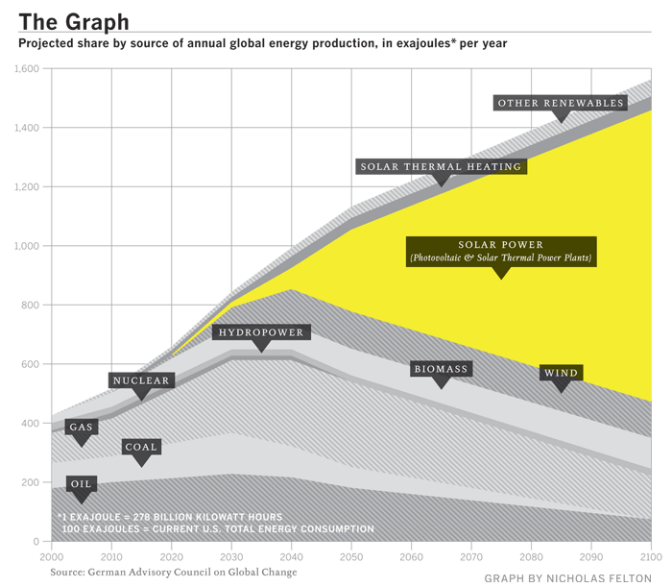
\includegraphics[width=0.95\columnwidth]{sample-graph.png}
\vfill\null
\columnbreak
\footnotesize
Nullam in urna lacinia orci consequat dictum. Nam scelerisque, nisl in euismod eleifend, justo diam bibendum dui, sed congue diam enim sit amet turpis. Suspendisse rhoncus felis nec lacus blandit mollis. Pellentesque lectus est, accumsan ac pellentesque aliquam, bibendum quis metus. Nunc interdum laoreet odio, eu feugiat velit feugiat sodales. Sed suscipit neque id dui dapibus non facilisis elit ultrices.
\vfill\null
\end{multicols}
\end{minipage}
}


\headerbox{RESULTS}
{name=results, span=1, column=1, row=0, below=abstract}{
\setlength{\parskip}{0.5em}

\begin{multicols}{2}

\small

Bus qui denis incimaio con reserum quamet aliquam re verspernam alias itatur? Qui sinullo ribuste empore ium ipitem rero miligente solupta temodi assequistium quidenis sene quide pore dolupta por modictur aga acienducid moluptate cum vellupta.

\begin{equation*}
\cos\mathopen{}\left(\frac{\omega t}{\sqrt{\alpha\gamma}}\right)\mathclose{} = \sum_{n=0}^\infty \frac{(-1)^{2n}}{(2n)!} \frac{(\omega t)^{2n}}{\alpha^{n}\gamma^{n}}
\end{equation*}



Ectatem pedicimpori re ellenducium et as ex eum fugia prateni con conest qui dolessi andae. Sitaspis earum rem ut dolor alignisci rerovid qui tem faccus nus, ut ab illiber ovitae. Es ad qui blat iliquis et estem fugia dolum sed quias enis dolorerrovid quiscia sus parumqu aecepra voluptur sum doluptatus molorporate vene volupta quia dolorec totatum hil illique ipsum debisimaio eatur maximi. 

\vfill\null
\columnbreak

Volupta nonsequiam vollit volenec eptiisqui odi tem faccus sequi ipsus excerum volut harions. Es ad qui blat iliquis et estem fugia dolum sed quias enis dolorerrovid quiscia.


\begin{center}
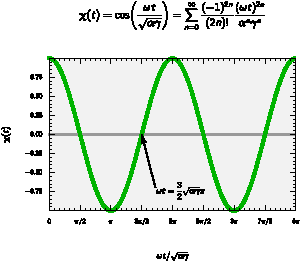
\includegraphics[scale=1,valign=T]{sample-figure.pdf}
\end{center}

\footnotesize \smaller
\textbf{Caption:} Graphics produced on Mathematica using MaTeX to make labels and other mathematics match the style of the maths in the poster.
\vfill\null
\end{multicols}

}

\headerbox{REFERENCES}
{name=references,span=1,column=1,below=results}{
Es ad qui blat iliquis et estem fugia dolum sed quias enis dolore rovid quiscia sus parumqu aecepra voluptur sum doluptatus molorporate vene volupta quia dolorec totatum hil illique ipsum debisimaio eatur maximi, volupta nonsequiam vollit volenec eptiisqui odi tem faccus sequi ipsus excerum volut harions.

\begin{enumerate}
\item Qui denis incimaio con reserum quamet
\item Qui sinullo ribuste mporeium ium ipitem rero miligente
\item Solupta temodi assequistium quidenis sequide pore
\item Dolupta por modictur acienducid moluptate cum
\item Vellupta es ad qui blat iliquis et estem fugia
\end{enumerate}
\vspace{1mm}
}






\headerbox{CONCLUSIONS}
{name=conclusions, span=1, column=0, row=0, below=background2,
 above=bottomlogos
 }{
\vspace{0.5mm}

\begin{itemize}
\item Aliquam posuere consectetur mi, ac imperdiet lectus auctor non.
Sed commodo posuere nisi, eu rutrum mauris gravida a.
\item Nunc imperdiet sagittis ante vitae elementum.
\item Mauris vel erat vitae nibh tincidunt auctor. In adipiscing vehicula
elementum. Quisque vel est nulla.
\end{itemize}
}

\headerbox{ACKNOWLEDGEMENTS}
{name=acknowledgements, span=1, column=1, below=references, 
above=bottomlogos
}{
\acknowledgementsfont
Qui denis incimaio con reserum quamet. Qui sinullo ribuste mporeium ium ipitem rero miligente. Solupta temodi assequistium quidenis sequide pore Dolupta por modictur acienducid moluptate cum Vellupta es ad qui blat iliquis et.
}




\end{poster}
\end{document}









